%! TEX root = part7.tex
% the main TeX file which is intended to compile, :VimtexReload after adjustment
% :h vimtex-tex-root
\documentclass[../gbr_teknik.tex]{subfiles}
% \includeonlyframes{current}
% \setbeameroption{hide notes} % Only slides
% \setbeameroption{show only notes} % Only notes
% \setbeameroption{show notes on second screen=right} % Both

\begin{document}

\section{Simbol Las}

\begin{frame}[mytitle=standard,t,mycolor=digiPH_white,light]\frametitle{Tujuan Pembelajaran}
	Setelah mempelajari materi ini, mahasiswa mampu:
	\begin{itemize}
		\item Mengidentifikasi bentuk-bentuk sambungan las
		\item Menafsirkan bentuk alur las
		\item Membaca lambang las pada gambar kerja
		\item Menggunakan lambang las pada gambar kerja
	\end{itemize}\end{frame}

\begin{frame}[mytitle=standard,c,mybg=bglight2,light]\frametitle{Pengertian Sambungan Las}
	\begin{itemize}
		\item Pengelasan adalah metode penyambungan permanen pada bagian mesin atau konstruksi
		\item Dibandingkan paku keling:
		      \begin{itemize}
			      \item Lebih ringan
			      \item Lebih kuat
		      \end{itemize}
		\item Digunakan secara luas dalam:
		      \begin{itemize}
			      \item Industri kecil
			      \item Industri besar
		      \end{itemize}
	\end{itemize}\end{frame}

\begin{frame}[mytitle=standard,t,mycolor=digiPH_uniblue,light]\frametitle{Bentuk Sambungan Las}
	\begin{itemize}
		\item Sambungan las memiliki beberapa bentuk dasar
		\item Digunakan sesuai kebutuhan konstruksi
	\end{itemize}\end{frame}

\begin{frame}[mytitle=standard,c,mycolor=digiPH_white,light]
	\frametitle{Bentuk Sambungan Las}
	\begin{center}
		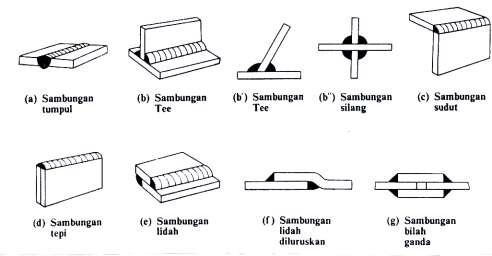
\includegraphics[width=.8\textwidth]{../figures/samb_las.jpg}
	\end{center}\end{frame}

\begin{frame}[mytitle=standard,c,mybg=bglight2,light]\frametitle{Pengertian Alur Las}
	\begin{itemize}
		\item Alur las digunakan untuk menampung cairan logam las
		\item Berfungsi menyatukan dua benda kerja
		\item Bentuk alur mempengaruhi:
		      \begin{itemize}
			      \item Kekuatan sambungan
			      \item Kualitas hasil las
		      \end{itemize}
	\end{itemize}\end{frame}

\begin{frame}[mytitle=standard,t,mycolor=digiPH_creamy,dark]
	\frametitle{Bentuk Alur Las}
	\begin{itemize}
		\item Terdapat berbagai bentuk alur las
		\item Pemilihan tergantung ketebalan dan jenis sambungan
	\end{itemize}\end{frame}

\begin{frame}[mytitle=standard,t,mycolor=digiPH_white,light]
	\frametitle{Bentuk Alur Las}
	\begin{center}
		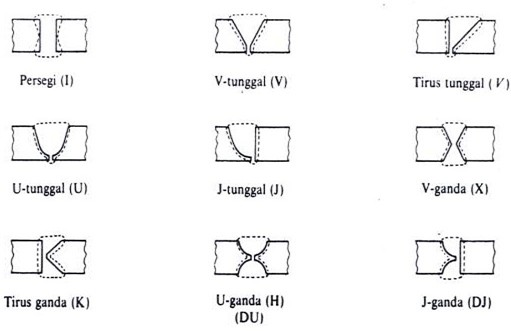
\includegraphics[width=.8\textwidth]{../figures/alur_las.jpg}
	\end{center}\end{frame}

\begin{frame}[mytitle=standard,c,mybg=bglight3,light]\frametitle{Lambang Las}
	\begin{itemize}
		\item Digunakan untuk menyederhanakan gambar teknik
		\item Memudahkan komunikasi antara:
		      \begin{itemize}
			      \item Perencana
			      \item Pelaksana (tukang las)
		      \end{itemize}
		\item Berlaku untuk:
		      \begin{itemize}
			      \item Las tunggal
			      \item Las dua sisi
		      \end{itemize}
	\end{itemize}\end{frame}

\begin{frame}[mytitle=standard,c,mycolor=digiPH_white,light]\frametitle{Jenis Lambang Las}
	\begin{center}
		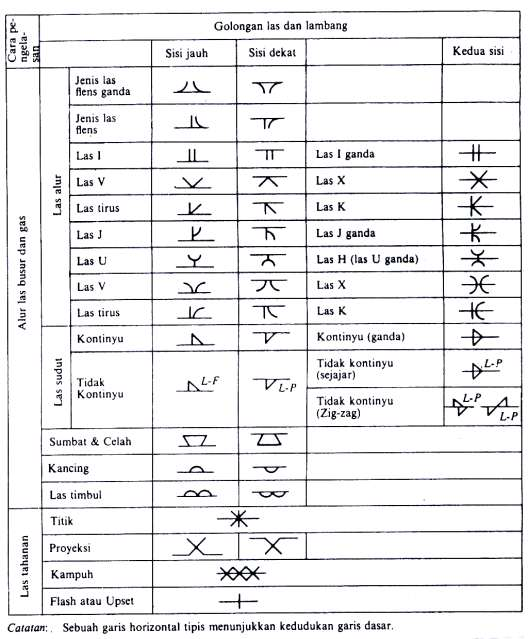
\includegraphics[height=.83\textheight]{../figures/lambang_las.jpeg}
	\end{center}\end{frame}

\begin{frame}[mytitle=standard,c,mycolor=digiPH_creamy,dark]\frametitle{Penggunaan Lambang Las}
	\begin{itemize}
		\item Lambang las digunakan dalam gambar kerja
		\item Menunjukkan:
		      \begin{itemize}
			      \item Jenis las
			      \item Lokasi las
			      \item Ukuran las
		      \end{itemize}
	\end{itemize}\end{frame}

\begin{frame}[mytitle=standard,c,mybg=bglight3,light]
	\frametitle{Penggunaan Simbol Las}
	\begin{center}
		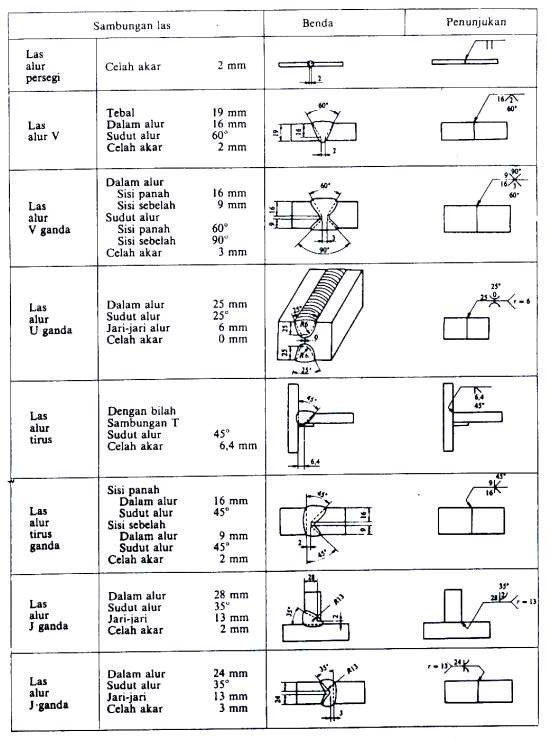
\includegraphics[height=.88\textheight]{../figures/penggunaan_las.jpg}
	\end{center}\end{frame}

\begin{frame}[mytitle=center,t,mybg=bglight1,light]\frametitle{Kesimpulan}
	\begin{itemize}
		\item Pengelasan adalah metode sambungan permanen yang kuat dan efisien
		\item Bentuk sambungan dan alur mempengaruhi kualitas las
		\item Lambang las penting dalam komunikasi gambar teknik
	\end{itemize}\end{frame}


\end{document}
